\section{Domain decomposition}
\label{sec_decomposition}

Run the previous program ({\tt 05-06-main.cpp}) in parallel on two processors. 
As a reminder, you do it with:
%
\begin{verbatim}
> mpiexec -np 2 ./Boil
\end{verbatim}
%
The program will create the following output:
%
{\small \begin{verbatim}
# Plotting: step-before_p000.dat
# Plotting: step-before_p001.dat
Domain level 3 created !
Domain level 2 created !
Domain level 1 created !
# Plotting: sca_p000.dat
# Plotting: vec_p000.dat
# Plotting: sca_p001.dat
# Plotting: vec_p001.dat
# Plotting: step-after_p000.dat
# Plotting: dom-after_p000.dat
# Plotting: step-after_p001.dat
# Plotting: dom-after_p001.dat
+==========================================
| Total execution time: 0.175 [s]
+------------------------------------------
| Time spent in plotting    : 0.13 [s]    (74.2857%)
| Time spent in bounding box: 0 [s]    (0%)
| Time spent in cell cutting: 0.015 [s]    (8.57143%)
| Time spent in flood fill  : 0.02 [s]    (11.4286%)
| Time spent elsewhere      : 0.01 [s]    (5.71429%)
+------------------------------------------
\end{verbatim}}
%
(Remember that domains are plotted implicitly, without direct invocation).
You get two domains, one for each processor. Namely, the grids are stored
in {\tt dom-after\_p000.dat} for processor~0 and {\tt dom-after\_p001.dat}
for processor~1. These two grids are shown in Fig.~\ref{fig_domain_decomp}.

%----------%
%          %
%  Domain  %
%          %
%----------%
\begin{figure}[ht]
  \centering
  \setlength{\unitlength}{1mm}
  \begin{picture}(130,47)(0,0)
    \thickbox{130}{47}
    \put( 0,-27){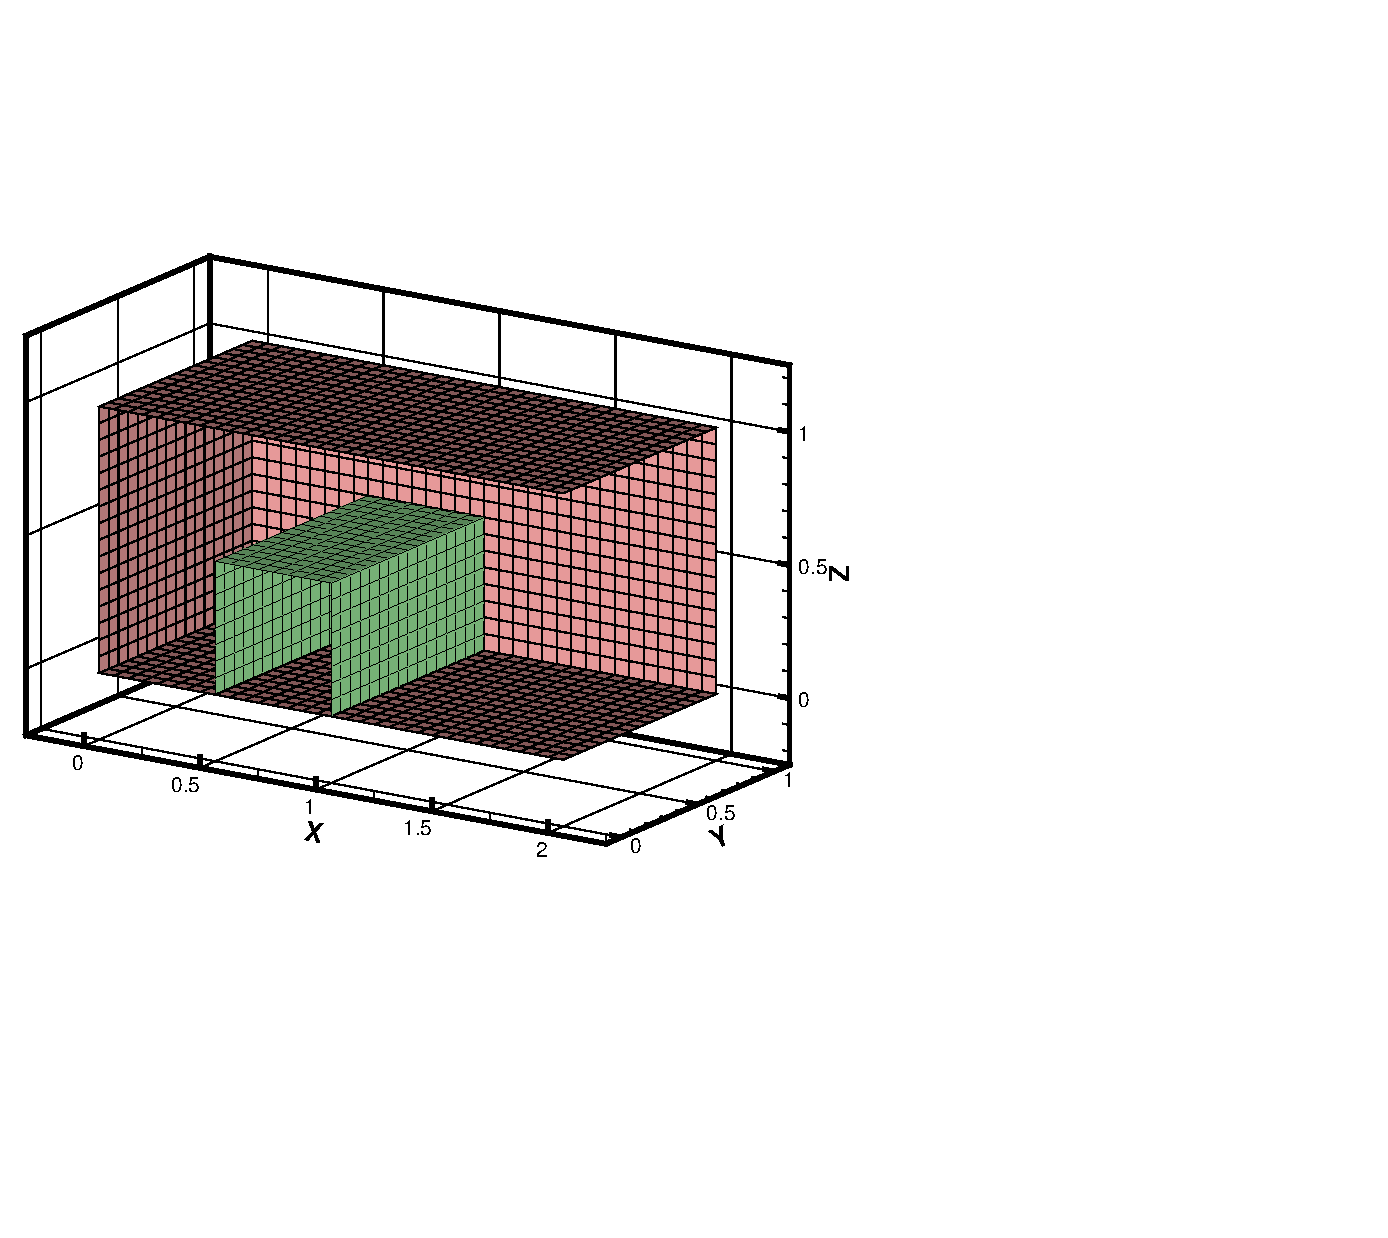
\includegraphics[scale=0.45]{Figures/05-10-par-0.eps}}
    \put(30,-21){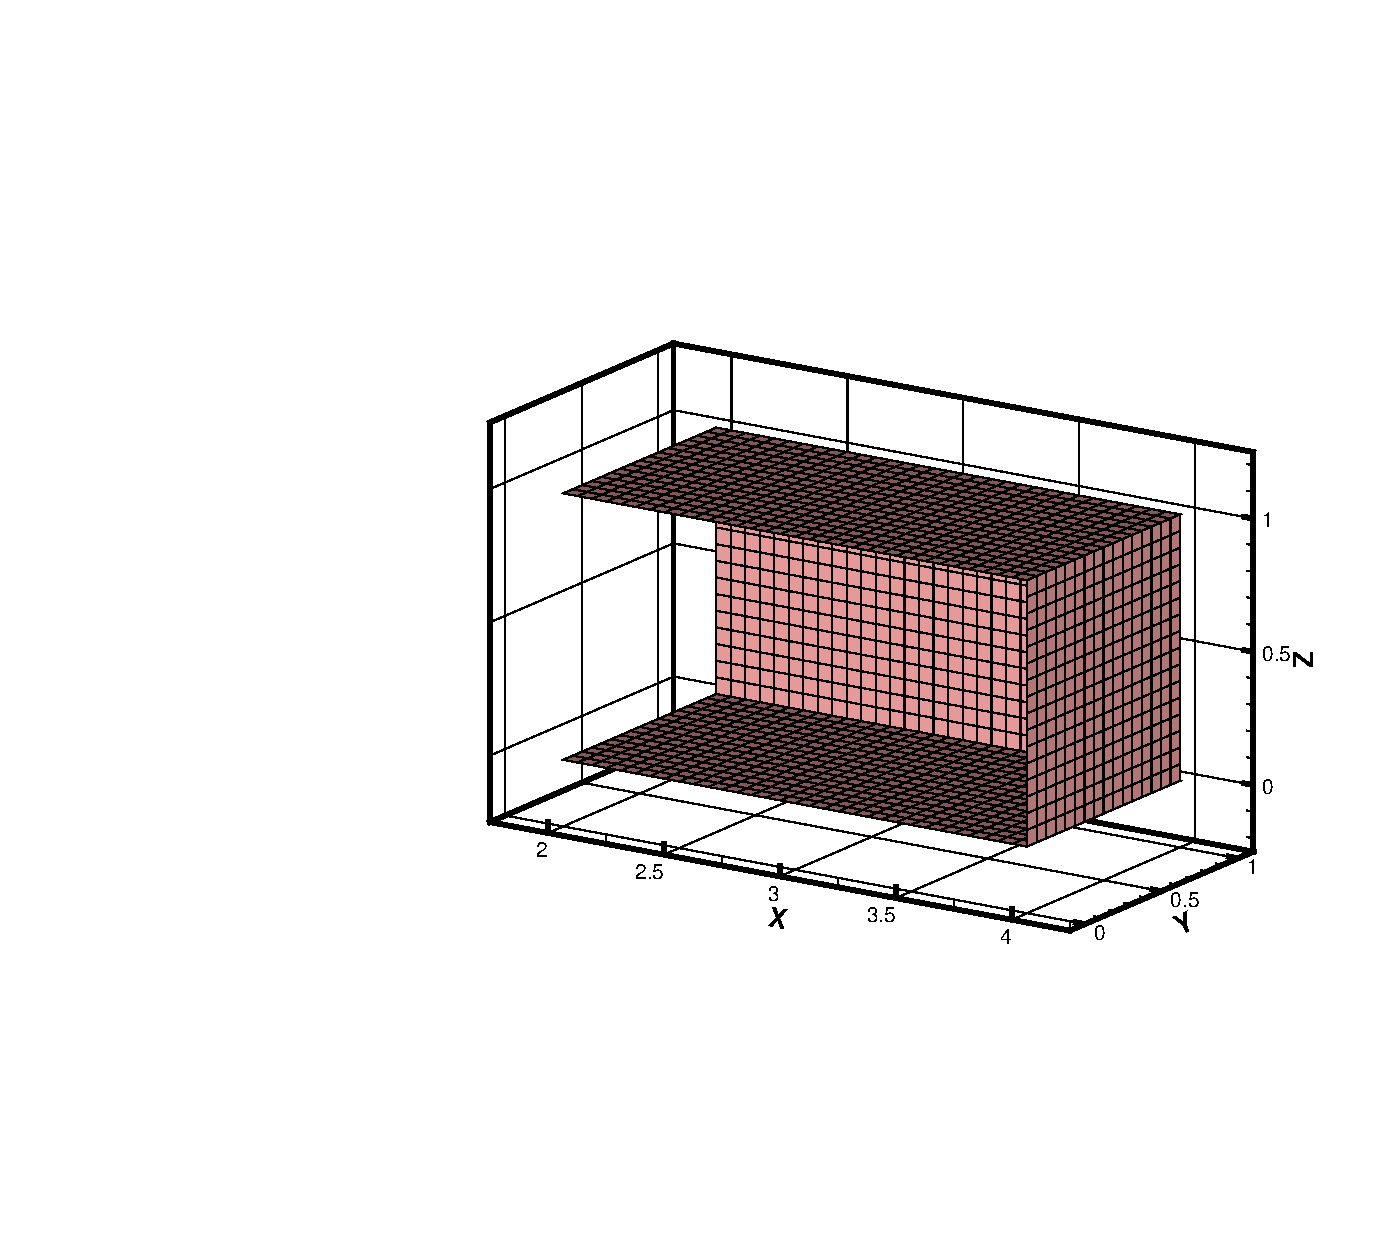
\includegraphics[scale=0.45]{Figures/05-10-par-1.eps}}
  \end{picture}
  \caption{Computational domain decomposed in two sub-domains.
           The front face, as well as the face between the sub-domains 
           are removed from the figure for the sake of clarity.}
  \label{fig_domain_decomp}
\end{figure}

While it is undoubtedly interesting to see the decomposed computational
domain, it is of little practical value. Much more often one wants to 
see the entire computational domain, together with solutions of governing
equations on it. {\psiboil}, if ran in parallel, plots as many domains
and result files as there were processors used. That is the simplest,
but also the most efficient way to parallelize file output. To connect
the files, we use an external program, called {\tt Connect}\footnote{It
was possible to create {\psiboil} in such a way that it creates a single
result file, no matter how many processors have been used. But, that would
put additional burden on parallel efficiency of {\psiboil}, only to make
post-processing more convenient for the user. It does not make sense to
sacrifice efficiency for convenience, particularly for an academic code
such as {\psiboil}, which is not meant to beat commercial CFD packages
in user-friendliness, or convenience.} 

{\tt Connect} is a part of {\psiboil} package, and resides in directory:
{\tt PSI-Boil/Src/Connect}, hereafter referred to as {\em connect}
directory. If you followed the instructions for creating
{\tt Makefile}s (Sec.~\ref{sub_sec_creating_makefiles}), there should 
already be a {\tt Makefile} in connect directory. Go there and run
{\tt make}. After a short compilation, an executable with the name 
{\tt Connect} is created. Go back to source and run:
%
\begin{verbatim}
> ./Connect/Connect
\end{verbatim}
%
It will print short message with outlining program usage, namely:
%
{\small \begin{verbatim}
Usage:
Connect/Connect <base_name> <ext> <number_of_processor> [time_step/level]
\end{verbatim}}
%
The first item being printed is the {\tt Connect} program name with full
path. It is followed by command line arguments, which are:
%
\begin{itemize}
  \item {\tt base\_name} - name assigned in call to plotting functions
        In the present case, it is {\tt domain}, implicitly defined
        by {\psiboil}.
  \item {\tt ext} - file extension, determining the file type being connected. 
        It may be either {\tt gmv} for GMV, or {\tt dat} for Tecplot. 
  \item {\tt number\_of\_processor} - clearly number of processors over which 
        the domain is distributed. For this case, it is~2. 
  \item {\tt time\_step/level} - the final argument which specifies the time 
        step, or grid level. This argument is optional, but for the present 
        case, grid level has to be specified. 
\end{itemize}
%
So, to connect the domain you got after the run on two processors, run:
%
\begin{verbatim}
> ./Connect/Connect dat dom 2 0
\end{verbatim}
%
and, after messages such as these:
%
{\small \begin{verbatim}
reading: dom-after_p000.dat
reading: dom-after_p001.dat
number of variables (excluding coordinates): 0
number of variables (excluding coordinates): 0
creating: dom-after.dat
body 0
present at 0
nodes 1664
cells 832
bodies finished
\end{verbatim}}
%
It will create the file {\tt dom-after.dat} which holds the single grid (not
distributed). 

%---------------------------------------------------------------------nutshell-%
\vspace*{5mm} \fbox{ \begin{minipage}[c] {0.97\textwidth} %-----------nutshell-%
    {\sf Section \ref{sec_decomposition} in a nutshell} \\  %---------nutshell-%
    
      - When ran in parallel, {\psiboil} automatically decomposes the
      the computational domain. \\

      - {\psiboil} performs separate plotting, i.e.\ each processors plots
      its own sub-domain. \\ 

      - Solid part is represented with {\tt Obstacle}s, while fluid
      is everywhere else. \\

      - Sub-domains are connected into a single file, using the program {\tt Connect},
      residing in directory {\tt PSI-Boil/Src/Connect}. \\

      - {\tt Connect} is not build by default. To build it, run {\tt make} in
      it's directory. 

  \end{minipage} } %--------------------------------------------------nutshell-%
%---------------------------------------------------------------------nutshell-%
